\documentclass[
    12pt,
    a4paper,
    addpoints,
    answers,
    convocatoria=ext,
    titulacion=CD,
    curso=2023/2024,
]{db-exam}

\begin{document}

\begin{questions}

% Bloque 1: Modelo Entidad/Relación y paso a tablas
\question{\textbf{Bloque ``Modelo Entidad/Relación y paso a tablas''}}

\begin{parts}
\part[3]

La organización \textit{Pokemon Masters Association} ha creado un sistema de registro para gestionar entrenadores y sus capturas en diversas localizaciones.

Estas localizaciones tienen un nombre único, y pertenecen a una y solo una de las diez regiones, también cada una con su nombre único. \textbf{Todas} las regiones poseen localizaciones. Los entrenadores son identificados por su alias único y se guarda su fecha de nacimiento. Los pokemons tienen un número único, nombre, y tipo, que puede ser Acero, Agua, Bicho, Dragón, Eléctrico, Fantasma, Fuego, Hada, Hielo, Normal, Planta, Psíquico, Roca, Siniestro, Tierra, Veneno y Volador; por cierto, no se conoce por el momento ninguno tipo Hada, pero no se descarta encontrarlo en un futuro, así que se mantiene el tipo en la base de datos.

Destacar que las localizaciones se caracterizan por atraer siempre a un tipo con mayor frecuencia, así que es interesante saber también cuál es ese tipo para cada localización; como antes, no se conoce ninguna localización que genere concretamente el tipo Hada.

Cada vez que un entrenador captura un pokémon de un número determinado, esta se registra junto con la fecha de la captura y el nivel de dicho pokemon. Esta información será única para cada combinación de entrenador, pokemon, localización y región.

\textbf{Realizar}:

\begin{itemize}
    \item Un modelo conceptual de datos mediante la técnica del \textbf{modelo Entidad-Relación de Chen} que modele el sistema de registro mencionado.
\end{itemize}


\begin{solution}
\begin{center}
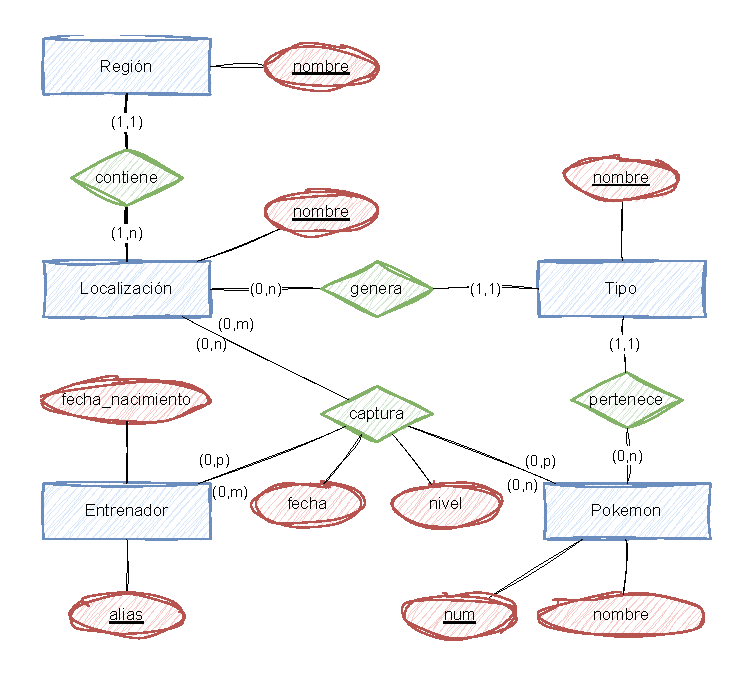
\includegraphics[width=.8\textwidth]{figs/bbdd-cdia-2023-2024-extraordinaria/2024-extraordinaria-gcdia-mer.pdf}
\end{center}
\end{solution}
\end{parts}


% SQL
\newpage
\question{\textbf{Bloque ``Lenguaje SQL''}}

Dado la siguiente creación de tablas en SQL:

\begin{lstlisting}[language=sql]
CREATE TABLE entrenadores (
    alias VARCHAR(50) UNIQUE NOT NULL,
    edad INT NOT NULL,
    PRIMARY KEY (alias)
);

CREATE TABLE pokemons (
    num INT UNIQUE NOT NULL,
    nombre VARCHAR(50) UNIQUE NOT NULL,
    tipo VARCHAR(50) NOT NULL,
    PRIMARY KEY (num)
);

CREATE TABLE localizaciones (
    nombre VARCHAR(50) UNIQUE NOT NULL,
    tipo   VARCHAR(50) NOT NULL,
    PRIMARY KEY (nombre)
);

CREATE TABLE capturas (
    entrenador VARCHAR(50) NOT NULL,
    pokemon INT UNIQUE NOT NULL,
    localizacion VARCHAR(50) NOT NULL,
    PRIMARY KEY (entrenador, pokemon, localizacion),
    CONSTRAINT fk_entrenador 
        FOREIGN KEY (entrenador) REFERENCES entrenadores (alias),
    CONSTRAINT fk_pokemon 
        FOREIGN KEY (pokemon) REFERENCES pokemons (num),
    CONSTRAINT fk_localizacion 
        FOREIGN KEY (localizacion) REFERENCES localizaciones (nombre)
);
\end{lstlisting}

Se pide:
\begin{parts}

% resta
\part[\half] Escriba una consulta en SQL que devuelva el \texttt{alias} de los entrenadores que nunca han capturado un pokemon en la \texttt{localizacion} `\textit{Monte Moon}'.

\begin{solution}[15em]
\begin{lstlisting}[language=sql]
SELECT alias
FROM entrenadores
WHERE alias NOT IN (SELECT entrenador
                     FROM capturas
                     WHERE localizacion = 'Monte Moon')
\end{lstlisting}
\end{solution}

% interseccion
\part[\half] Escriba una consulta en SQL que devuelva el \texttt{nombre} de los pokemons que han sido capturados por los entrenadores `\textit{Ash Ketchum}' y `\textit{Gary Oak}'.

\begin{solution}[15em]
\begin{lstlisting}[language=sql]
SELECT nombre
FROM pokemons
WHERE num IN (SELECT pokemon
              FROM capturas
              WHERE entrenador = 'Ash Ketchum')
  AND num IN (SELECT pokemon
              FROM capturas
              WHERE entrenador = 'gary Oak')         
\end{lstlisting}
\end{solution}

% division
\part[\half] Escriba una consulta en SQL que devuelva el \texttt{alias} de los entrenadores que se hayan capturado todos los pokemon de \texttt{tipo} `\textit{fuego}'.

\begin{solution}[15em]
\begin{lstlisting}[language=sql]
SELECT alias
FROM entrenadores
WHERE NOT EXISTS (SELECT *
                  FROM pokemons
                  WHERE tipo = 'fuego'
                    AND NOT EXISTS (SELECT *
                                    FROM capturas
                                    WHERE capturas.pokemon = 
                                            pokemons.num
                                      AND capturas.entrenador = 
                                            entrenadores.nombre))
\end{lstlisting}
\end{solution}

% maximo
\part[\half] Escriba una consulta en SQL que devuelva el \texttt{nombre} de la localización o localizaciones donde más pokemons se han capturado.

\begin{solution}[15em]
\begin{lstlisting}[language=sql]
SELECT localizacion
FROM capturas
GROUP BY localizacion
HAVING COUNT(*) >= ALL (SELECT COUNT(*)
                        FROM capturas
                        GROUP BY localizacion);
\end{lstlisting}
\end{solution}

% minimo
\part[\half] Escriba una consulta en SQL que devuelva el \texttt{tipo} (o \texttt{tipos}) de pokemons del que existen menos pokemons.

\begin{solution}[15em]
\begin{lstlisting}[language=sql]
SELECT tipo
FROM pokemons
GROUP BY tipo
HAVING COUNT(*) <= ALL (SELECT COUNT(*)
                        FROM pokemons
                        GROUP BY tipo);
\end{lstlisting}
\end{solution}

% joins
\part[\half] Escriba una consulta en SQL que devuelva el \texttt{alias} de los entrenadores que hayan capturado el pokemon denominado \textit{New} en la localización `\textit{Cueva Celeste}'.

\begin{solution}[15em]
\begin{lstlisting}[language=sql]
SELECT DISTINCT alias
FROM capturas
    INNER JOIN pokemons ON pokemons.num = captura.pokemon
WHERE nombre = 'New'
  AND localizacion = 'Cueva Celeste';
\end{lstlisting}
\end{solution}

% procedmiento
\part[1] Escriba un procedimiento almacenado en SQL que dado el \texttt{nombre} de un pokemon, que se pasará como parámetro de entrada, liste por pantalla el número de veces que ha sido capturado en cada localización. Si un pokemon nunca ha sido capturado no es necesario que aparezca en el listado. El listado debe aparecer ordenador de mayor a menor número de capturas.

\begin{solution}[15em]
\begin{lstlisting}[language=sql]
DELIMITER $$
CREATE PROCEDURE num_veces_capturado (IN nombre_pokemon VARCHAR(50))
BEGIN
    SELECT localizacion, COUNT(*) AS num_capturas
    FROM capturas
        INNER JOIN pokemons ON pokemons.num = capturas.pokemon
    WHERE nombre = nombre_pokemon
    GROUP BY localizacion
    ORDER BY num_capturas DESC;
END$$
DELIMITER ;
\end{lstlisting}
\end{solution}

% trigger
\part[1] Escriba un \textit{trigger} en SQL que impida que los entrenadores menores de 16 años que añadan nuevas capturas de pokemons de \texttt{tipo} `\textit{fuego}' para evitar sufrir quemaduras.

\begin{solution}[15em]
\begin{lstlisting}[language=sql]
DELIMITER $$
CREATE TRIGGER evita_fuego_16 BEFORE INSERT ON pokemons 
FOR EACH ROW
BEGIN
    DECLARE e INTEGER;
    DECLARE t VARCHAR(50);

    SELECT edad INTO e 
    FROM entrenadores
    WHERE alias = NEW.entrenador;

    SELECT tipo INTO t
    FROM pokemons
    WHERE num = NEW.pokemon;

    IF e < 16 AND tipo = 'fuego' THEN
        SIGNAL SQLSTATE '162342'
        SET MESSAGE_TEXT = 'Los entrenadores menores de 16 años
        no pueden capturar pokemons de tipo fuego';
    END IF;
END$$
DELIMITER ;
\end{lstlisting}
\end{solution}

% permisos de usuario
\part[\half] Cree un usuario denominado `\textit{cartógrafo}' y otórguele permisos de consulta e inserción sobre la tabla \texttt{localizaciones}. A continuación, inserte una nueva localización denominada `\textit{Pueblo Paleta}' de tipo `\textit{ciudad}'.

\begin{solution}[12em]
\begin{lstlisting}[language=sql]

CREATE USER 'cartógrafo' IDENTIFIED BY '1234';

GRANT SELECT, INSERT ON localizaciones TO 'cartógrafo';

INSERT INTO localizaciones VALUES ("Pueblo Paleta", "Ciudad");
\end{lstlisting}
\end{solution}

\end{parts}


% Bloque Acceso programático
\newpage
\question{\textbf{Bloque ``Acceso programático''}}

\begin{parts}
\part[1] Tomando como punto de partida un \texttt{SCHEMA} de bases de datos basado en el modelo relacional del bloque anterior, complete los huecos del siguiente código fuente en \texttt{python} de tal manera que se satisfaga la funcionalidad indicada como comentarios.

\begin{lstlisting}[language=python]
import mysql.connector

# establecimiento de conexion
mydb = mysql.connector.connect(
  host='localhost',
  user='root',
  password='root',
  database='pokemon_db',
)

cursor = mydb.cursor()

# Añadir entrenador
alias = 'Ash Ketchum'
edad = 10

cursor.execute(
    'INSERT INTO entrenadores _________________________________',
    (alias, edad)
)

mydb.commit()

# Listar los nombres y tipos de los pokémons capturados en una
# localización específica
localizacion_buscada = 'Bosque Verde'
consulta = '''
SELECT p.nombre, p.tipo 
FROM pokemons p
JOIN capturas c ON p.num = c.pokemon
WHERE c.localizacion = %s
'''

cursor.______________(________________________________________________)

for (nombre_pokemon, tipo_pokemon) in cursor:
    print(f'{nombre_pokemon} ({tipo_pokemon})')

# Cierre de recursos
cursor.close()
cnx.close()
mydb.close()
\end{lstlisting}

\begin{solution}[1em]
\begin{lstlisting}[language=python]
import mysql.connector

# establecimiento de conexion
mydb = mysql.connector.connect(
  host='localhost',
  user='root',
  password='root',
  database='pokemon_db',
)

cursor = mydb.cursor()

# Añadir entrenador
alias = 'Ash Ketchum'
edad = 10

cursor.execute(
    'INSERT INTO entrenadores (alias, edad) VALUES (%s, %s)',
    (alias, edad)
)

mydb.commit()

# Listar los nombres y tipos de los pokémons capturados en una localización específica
localizacion_buscada = 'Bosque Verde'
consulta = '''
SELECT p.nombre, p.tipo 
FROM pokemons p
JOIN capturas c ON p.num = c.pokemon
WHERE c.localizacion = %s
'''

cursor.execute(consulta, (localizacion_buscada,))

for (nombre_pokemon, tipo_pokemon) in cursor:
    print(f'{nombre_pokemon} ({tipo_pokemon})')

# Cierre de recursos
cursor.close()
cnx.close()
mydb.close()
\end{lstlisting}
\end{solution}

\end{parts}

% Bloque Modelo relacional
\newpage
\question{\textbf{Bloque ``Modelo relacional''}}

\begin{parts}

\part[\half] ¿Qué pasos deberían darse para que la base de datos siguiente cumpliera la primera forma normal (1FN)?
    
  \vspace{1em}
    
  \begin{tabular}{lllll}
    \hline
    ID & Nombre & Edad & Ciudad & Pokemon \\
    \hline
    1 & Ash & 15 & Pueblo Paleta & Pikachu, Bulbasaur, Charmander \\
    2 & Misty & 13 & Ciudad Celeste & Psyduck, Starmie \\
    3 & Brock & 16 & Ciudad Plateada & Onix, Geodude, Zubat \\
    \hline
  \end{tabular}  
    
  \begin{solutionorbox}
    Actualmente existe más de un valor para el atributo \texttt{Pokemon}, por lo que se debería crear una nueva tabla que guardase \texttt{ID}, \texttt{Pokemon} para evitar que esto sucediera. En la tabla actual habría que eliminar la columna \texttt{Pokemon}.
  \end{solutionorbox}
\end{parts}

\end{questions}
\end{document}
